\section{Basic usage}

\subsection{Installation notes}

After successfully compiling CPlantBox the Python library \emph{plantbox} should be available on the system. 
Additionally, you will need the following Python packages: numpy, scipy, matplotlib, and vtk (e.g. pip3 install numpy). 

The figures of the rootsystem were created using Paraview, and some Paraview Python scripts for convenience.

\subsection{Small example}

The first example shows how to use CPlantBox: open a parameter file (L12), do the simulation (L18), and save the result (L21). 

\lstinputlisting[language=Python, caption=Example 1a]{../../examples/python/example1a_small.py} % basicstyle=\footnotesize, 

\noindent 
Lets revise the above code in more detail: 
\begin{itemize}
 \item[4] Imports the CPlantBox Python library (py\_plantbox) and name it pb.
 \item[7] Constructs the root system object.
 \item[12] Opens an .xml containing parameters describing the types of root (RootRandomParameters), and the type of pant (SeedRandomParameters). Alternatively, all parameter can be set or modified directly in Python (see Section \ref{sec:sa}).
 \item[15] Initializes the simulation: Creates the tap root the base roots (i.e. all basal roots, and shoot borne roots that might emerge), creates the tropisms and passes the domain geometry to it, and creates the elongation functions. 
 \item[18] Performs the simulation. The value 30 is the simulation time in days. If no simulation time is passed the simulation time is taken from the .pparam file. Note that simulation results are independent from the time step, i.e. 30 simulate(1) calls should yield the same result as simulate(30). 
 \item[21] Saves the resulting root system geometry in the VTK Polygonal Data format (VTP) as polylines, see Figure \ref{fig:basicA}. 
\end{itemize}

\subsection{Growth in a container}

This is an extension of the previous example, where the root system grows in one of two containers (a soil core or rectangular rhizotron). Such geometries are important if we want to mimic experimental settings. In CPlantBox the domain geometry is represented in a mesh free way using signed distance functions (SDF). A SDF returns the distance to the closest boundary, with negative sign if it lies inside of the domain, and a positive if it the point is outside.

\lstinputlisting[language=Python, caption=Example 1b]{../../examples/python/example1b_container.py}

The geometry is first created by constructing some specialization of the class SignedDistanceFunction, and is passed to the root system by the method setGeometry: 
\begin{itemize}
 \item[16] Construct a soil core. 
 \item[19] Construct a rhizotron.
 \item[22] Pick one of the two geometries. Note that it is important to call setGeometry before initialize.
 \item[34] Its possible to save the geometry as Paraview Python script for visualization (and debugging), see Figure \ref{fig:basicB}. Run this script in Paraview by Tools$\rightarrow$Python Shell, Run Script.
\end{itemize}

\begin{figure}
\begin{subfigure}[c]{0.5\textwidth}
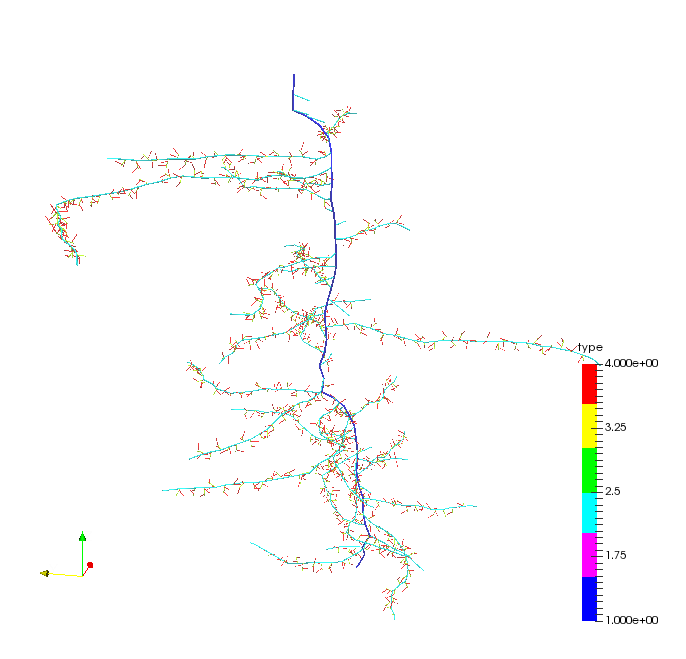
\includegraphics[width=0.99\textwidth]{example_1a.png}
\subcaption{Unconfined growth (Example 1a)} \label{fig:basicA}
\end{subfigure}
\begin{subfigure}[c]{0.5\textwidth}
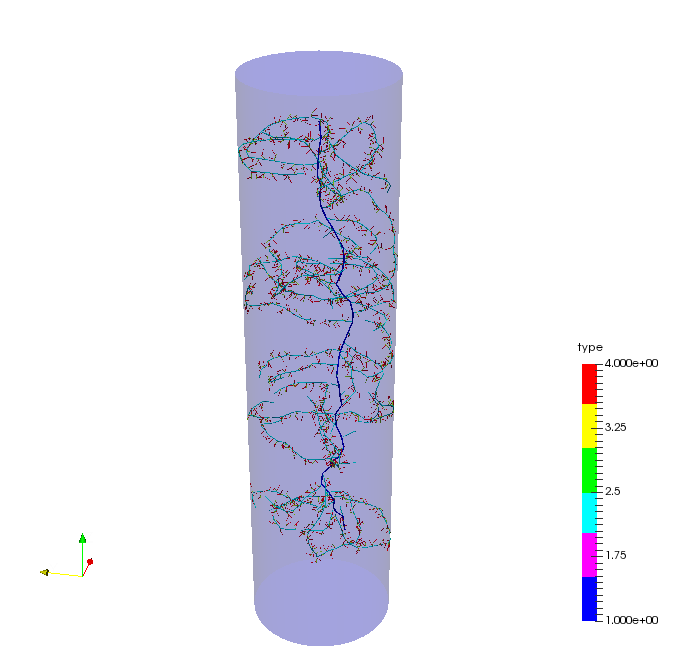
\includegraphics[width=0.99\textwidth]{example_1b.png}
\subcaption{Confined growth (Example 1b)} \label{fig:basicB}
\end{subfigure}
\caption{Resulting figures from Section 1} 
\end{figure}

Now, we show how to build more complex container geometries using SDF, 
furthermore, we show an example with multiple root systems that is computed in parallel.

\subsection{Using SDF with set operations}

In the following example we create more complex geometries that we might encounter in experiments. 
First, we show how to rotate a rhizotron (e.g. to see more roots at the wall due to gravitropism). 
Second, we create a split box experiment, and furthermore, an example where rhizotubes act as obstacles.

The following examples show how to build a complex geometry using rotations, translations and set operations on the SDF.

\lstinputlisting[language=Python, caption=Example 2a]{../../examples/python/example1c_complexcontainer.py}

\begin{itemize}

\item[14-20] Definition of a rotated rhizotron, see Figure \ref{fig:rhizo}: L16 creates the flat container with a small height, this container is then rotated and translated into the desired position. 
L17 is the position where the origin will lie, and L18 the rotational matrix around the x-axis. 
In L19 the origin position is rotated. Finally, in L20 the new rotated and translated geometry is created. 
\item[22-31] Definition of of a split box, see Figure \ref{fig:split}: The split box is composed of a left box, a right box, and a top box connecting left and right. In L31 the geometry is defined by the set operation union of the three compartments. 
\item[33-48] Definition of rhizotubes as obstacles, see Figure \ref{fig:rhizotubes}: L34 is the surrounding box, L35 a single rhizotube, that is rotated around the y-axis in L36. L38-L45 create a list of rhizotubes at different locations that mimics the experimental setup. 
L48 and L48 compose the final geometry by to set operation, first a union of all tubes, and then cut them out the surrounding box by taking the difference. 
\item[51] Pick one of the three geometries for your simulation.
\item[61] Also more complex geometries can be visualized by the Paraview script, however set operations are not really performed, only the involved geometries are visualized.

\end{itemize}

\begin{figure}
\begin{subfigure}[c]{0.3\textwidth}
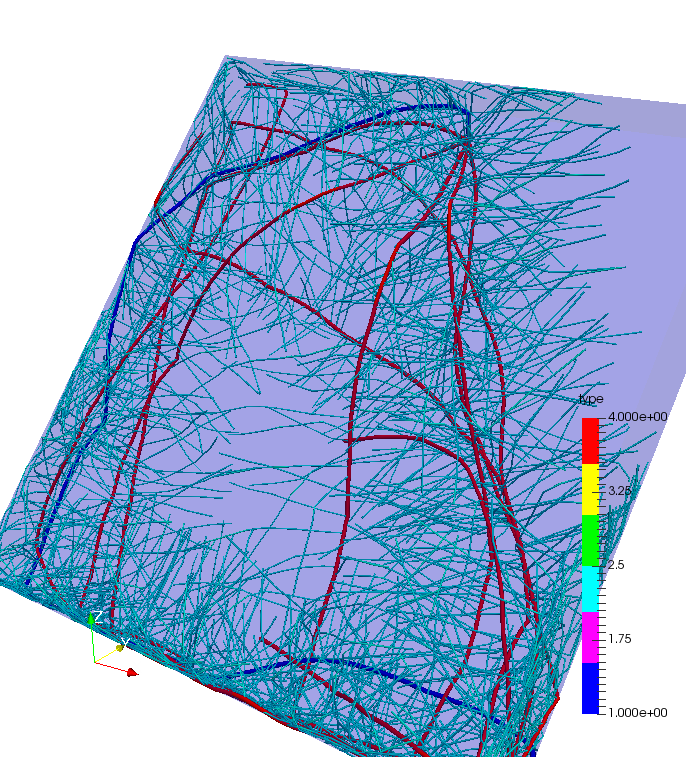
\includegraphics[width=0.99\textwidth]{example_2a1.png}
\subcaption{Rotated rhizotron} \label{fig:rhizo}
\end{subfigure}
\begin{subfigure}[c]{0.3\textwidth}
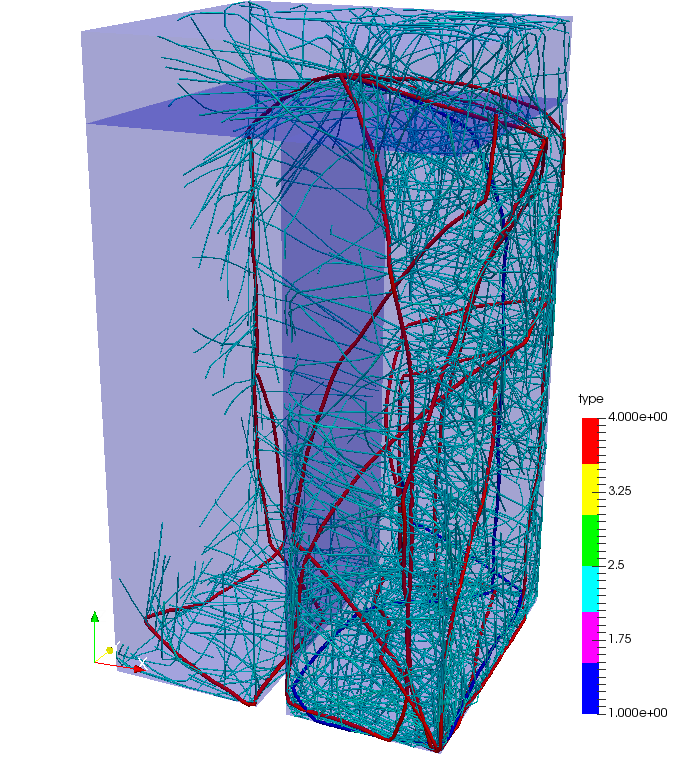
\includegraphics[width=0.99\textwidth]{example_2a2.png}
\subcaption{Split box} \label{fig:split}
\end{subfigure}
\begin{subfigure}[c]{0.3\textwidth}
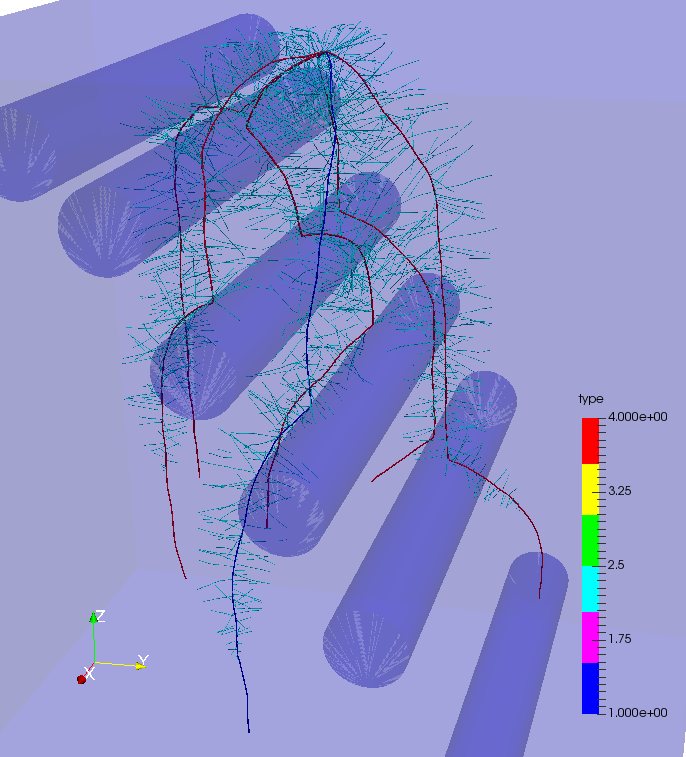
\includegraphics[width=0.99\textwidth]{example_2a3.png}
\subcaption{Rhizotubes} \label{fig:rhizotubes}
\end{subfigure}
\caption{Different geometries described by SDF (Example 2a)}
\end{figure}

\subsection{Multiple root systems}

Its possible to simulate multiple root systems. In the following we show a small plot scale simulation.

\lstinputlisting[language=Python, caption=Example 2b]{../../examples/python/example1d_multiple.py}

\begin{itemize}

\item[10,11] Set the number of columns and rows of the plot, and the distance between the root systems.

\item[14-21] Creates the root systems, and puts them into a list allRS. L19 sets the position of the seed. 

\item[24,25] Simulate all root systems 

\item[28-35] Saves each root systems, and additionally, saves all root systems into a single file. 
Therefore, we create an SegmentAnalyser object in L28 and merge all segments into it L32, and finally export the single file L35. The resulting geometry is shown in Figure \ref{fig:multiple}.

\end{itemize}

\begin{figure}
\centering
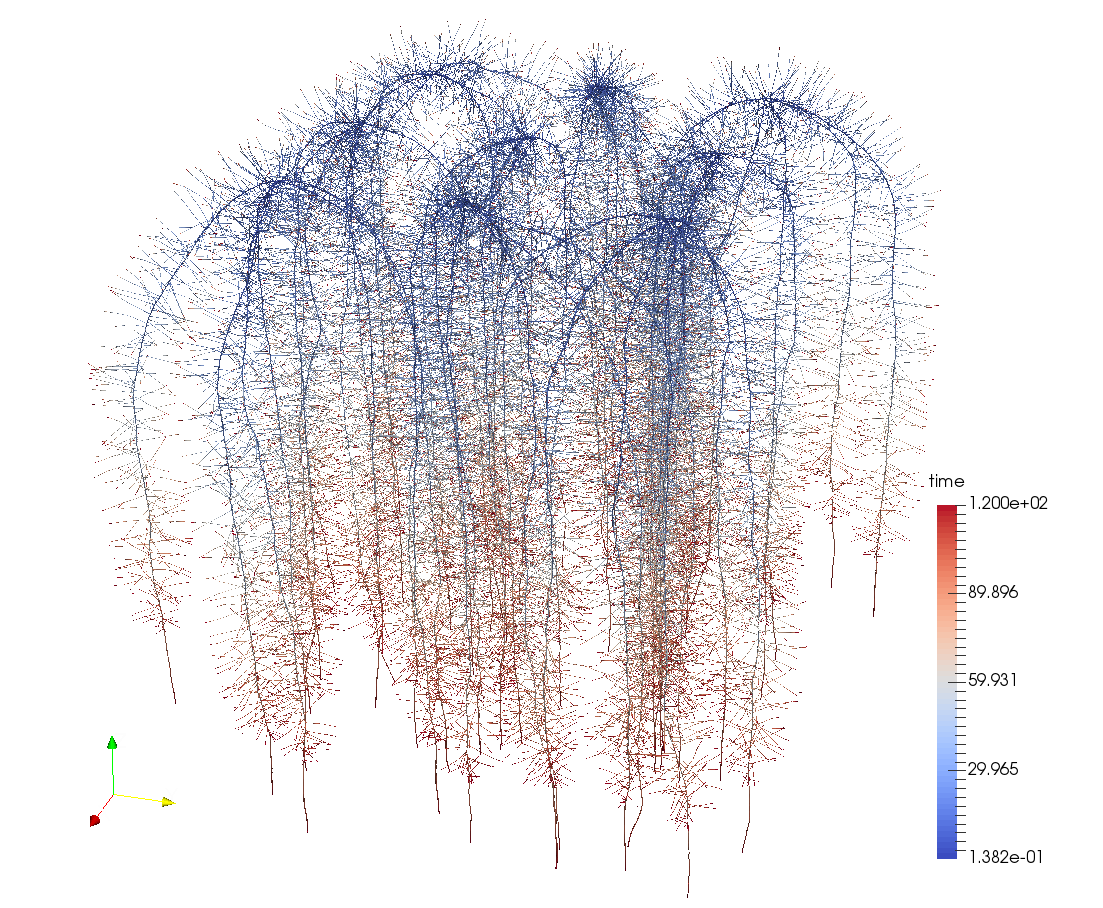
\includegraphics[width=0.7\textwidth]{example_2b.png}
\caption{Multiple root systems (Example 2b), colors denote the creation time of the root segments} \label{fig:multiple}
\end{figure}

Each root system has its own random number generator. By default the seed of the generator is initialized with the system clock. 
If this is not sufficient, e.g. if multiple root systems are initiated at the same time on multi-core systems, or the simulation shall be reproducable, the seed can be set manually using the method RootSystem::setSeed(int).



